\documentclass[11pt,a4paper]{article}

\usepackage[utf8]{inputenc}
\usepackage[T1]{fontenc}
\usepackage[brazil]{babel}
\usepackage[a4paper,top=1.6cm,bottom=1.6cm,left=1.7cm,right=1.7cm]{geometry}
\usepackage{microtype}
\usepackage{booktabs}
\usepackage{array}
\usepackage{tabularx}
\usepackage{enumitem}
\usepackage{titlesec}
\usepackage{xcolor}
\usepackage{parskip}
\usepackage{fancyhdr}
\usepackage{graphicx}
\usepackage{hyperref}
\usepackage{xurl}

\definecolor{azulmls}{RGB}{20,70,110}
\definecolor{cinzatexto}{RGB}{60,60,60}
\definecolor{verdeF}{RGB}{30,120,70}
\definecolor{vermelhoL}{RGB}{180,60,50}

\hypersetup{colorlinks=true, linkcolor=azulmls, urlcolor=azulmls}
\pagestyle{fancy}\fancyhf{}
\renewcommand{\headrulewidth}{0.4pt}
\lhead{\footnotesize\color{cinzatexto} MLS 2026.2 \textperiodcentered{} Projeto aplicado de extensão}
\rhead{\footnotesize\color{cinzatexto} Entrega 4 \textperiodcentered{} Dados e baseline}
\cfoot{\footnotesize\color{cinzatexto}\thepage}

\titleformat{\section}{\large\bfseries\color{azulmls}}{\thesection.}{0.5em}{}
\titleformat{\subsection}{\normalsize\bfseries\color{azulmls}}{}{0em}{}
\titlespacing*{\section}{0pt}{8pt}{3pt}
\titlespacing*{\subsection}{0pt}{6pt}{2pt}
\setlength{\parskip}{3pt}
\setlist[itemize]{leftmargin=1.4em, itemsep=1pt, topsep=1pt}

\newcommand{\sm}{\textbf{\textcolor{verdeF}{Sim}}}
\newcommand{\nao}{\textbf{\textcolor{vermelhoL}{Não}}}

\begin{document}

\begin{center}
    {\LARGE\bfseries\color{azulmls} Contrato de dados, repositório e baseline}\\[3pt]
    {\large Entrega 4 --- Aprendizagem de Máquina Supervisionada}\\[2pt]
    {\normalsize UFPB \textperiodcentered{} CCSA \textperiodcentered{} Ciência de Dados para Negócios \textperiodcentered{} 2026.2}
\end{center}
\vspace{3pt}\hrule\vspace{6pt}

\noindent\textbf{Equipe F:} Brenno Henrique Alves da Silva Costa; Gustavo Henrique Rocha Oliveira; Iasmin Vieira de Lima. \quad \textbf{Data:} 22/10/2026.\\
\textbf{Repositório:} \url{https://github.com/brennohdev/hu-demand-forecasting}\\
\textbf{Notebook:} \url{https://github.com/brennohdev/hu-demand-forecasting/blob/main/notebooks/auditoria_baseline.ipynb}

% ============================================================
\section{Contexto e objetivo}
Após a escuta no HU-UFPB (Entrega 3), o recorte passou a ser a \textbf{previsão de demanda de antimicrobianos}. A farmácia controla, em planilha manual, os tratamentos ativos para garantir que nenhum paciente fique sem o medicamento no meio do tratamento. A decisão apoiada é \textbf{quanto de cada antimicrobiano reservar/repor para o próximo mês}. Esta entrega produz a base analítica, o diagnóstico de qualidade, a partição e o baseline.

% ============================================================
\section{Contrato de dados}
\begin{tabularx}{\textwidth}{@{}>{\bfseries}p{3.4cm} X@{}}
\toprule
Chave e unidade & Um \textbf{tratamento} de um paciente com um antimicrobiano (uma linha). \\
Granularidade & Tratamento; agregado para \textbf{princípio ativo $\times$ mês} na modelagem de demanda. \\
Cobertura & 2025-03 a 2026-10; 7.425 tratamentos; 32 antimicrobianos; 17 setores. \\
Alvo & Demanda mensal (soma de \texttt{qtd\_total}) por antimicrobiano; fonte: planilha de tratamento (AGHU). \\
Corte temporal & Fechamento do mês: prevê-se a demanda do mês seguinte. \\
Atualização & A planilha é atualizada ao menos uma vez por dia na origem. \\
Restrições & Dado operacional do hospital; nome do paciente já anonimizado; não redistribuível; uso acadêmico. \\
\bottomrule
\end{tabularx}

% ============================================================
\section{Relatório de qualidade}
Principais problemas encontrados e decisões aplicadas (contagens antes/depois registradas no notebook):

\begin{tabularx}{\textwidth}{@{}p{3.3cm} X p{3.4cm}@{}}
\toprule
\textbf{Variável/base} & \textbf{Problema e decisão} & \textbf{Impacto} \\
\midrule
\texttt{qtd\_resta} & 99,8\% ausente; sem informação útil. Removida. & Nenhuma perda de sinal. \\
\texttt{qtd\_dispensada} & 98,3\% ausente. Removida. & Idem. \\
\texttt{suspender} & 78,7\% ausente; ausência significa ``não suspenso''. Convertida em flag binária. & Mantém o sinal sem imputar falso. \\
linhas duplicadas & 164 linhas idênticas. Removidas. & Evita contagem dobrada de demanda. \\
\texttt{data\_inicio} ausente & Poucas linhas sem data. Removidas (não entram na série). & Série temporal consistente. \\
mês 2026-10 & Coleta em 22/10: mês incompleto (demanda cai artificialmente). Excluído da modelagem. & Evita viés na métrica. \\
\texttt{setor} & Variações de grafia (ex.: espaços). Normalizado (maiúsculas, espaços). & Categorias consistentes. \\
\bottomrule
\end{tabularx}

\textbf{Observações:} a demanda mensal total é estável (faixa de 12 a 18 mil unidades/mês). A situação dos tratamentos é 78\% encerrada, 20\% suspensa e 2\% em andamento; a suspensão é um fenômeno frequente e candidato a alvo futuro (risco de interrupção).

% ============================================================
\section{Diagnóstico de vazamento}
Corte: previsão no fechamento do mês para o mês seguinte. Classificação de variáveis:

\begin{tabularx}{\textwidth}{@{}>{\raggedright\arraybackslash}p{3.9cm} c X@{}}
\toprule
\textbf{Variável} & \textbf{Permitida?} & \textbf{Justificativa (relação com o corte)} \\
\midrule
\texttt{principio\_ativo} & \sm & característica estável do item, conhecida antes do corte. \\
\texttt{setor} & \sm & definida na prescrição; existe antes do corte. \\
mês do ano (sazonalidade) & \sm & derivada da data de início; não usa o futuro. \\
lags de \texttt{qtd\_total} & \sm & usa apenas meses anteriores já encerrados. \\
\texttt{data\_termino} & \nao & vazamento temporal: só conhecida após o fim do tratamento. \\
\texttt{situacao} & \nao & vazamento de alvo: é o desfecho, só existe depois. \\
\texttt{qtd\_dispensada}, \texttt{qtd\_resta} & \nao & consequência da decisão: registradas conforme o consumo ocorre. \\
\bottomrule
\end{tabularx}

\textbf{Consequência da decisão.} Variáveis como \texttt{situacao} e \texttt{qtd\_dispensada} parecem ótimas preditoras, mas só existem porque o tratamento já aconteceu; em produção não estariam disponíveis no corte. Por isso são proibidas.

% ============================================================
\section{Partição e baseline}
\textbf{Estratégia: temporal.} Como a decisão é aplicada ao futuro, o teste são os últimos meses, não um sorteio aleatório. \emph{Cenário imitado:} ``no fim de cada mês, prever a demanda do mês seguinte.''
\begin{itemize}
    \item Treino: 2025-03 a 2026-05 (15 meses). \quad Teste: 2026-06 a 2026-09 (4 meses).
    \item Pré-processamento (quando o modelo entrar) será ajustado só no treino, dentro de \texttt{Pipeline}, aplicando \texttt{transform} a validação/teste.
\end{itemize}

\textbf{Baselines (métrica no conjunto de teste):}

\begin{center}
\begin{tabular}{@{}lcc@{}}
\toprule
\textbf{Baseline} & \textbf{MAPE} & \textbf{MAE} \\
\midrule
Trivial (média do treino) & \textbf{9,6\%} & 1.478 \\
Operacional (persistência: repor como no mês anterior) & 15,8\% & 2.262 \\
\bottomrule
\end{tabular}
\end{center}

\textbf{Métrica escolhida:} MAPE (erro percentual de demanda), por ser interpretável para a farmácia e coerente com a decisão de reposição. \textbf{Número de referência do semestre: MAPE $\approx$ 9,6\%}; a demanda é estável, então qualquer modelo precisa superar a média para justificar complexidade.

\begin{center}
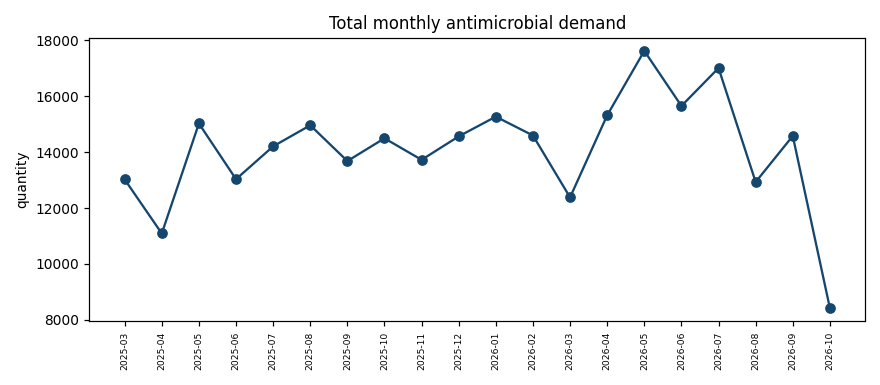
\includegraphics[width=0.86\textwidth]{../../figuras/g2_demanda_mensal.png}
\end{center}

% ============================================================
\section{Reprodutibilidade e verificação individual}
O notebook \texttt{notebooks/auditoria\_baseline.ipynb} executa do início ao fim (via \texttt{make notebook} / \texttt{uv}), apoiado no pacote \texttt{huforecast} (camadas: ingestão, processamento, features, modelagem), sem edição manual nem caminhos absolutos. Os dados brutos não são versionados (ver \texttt{.gitignore} e \texttt{data/raw/README.md}).

\textbf{Verificação individual (diagnóstico de 3 variáveis por integrante):}
\begin{itemize}
    \item \textbf{Brenno} --- \texttt{principio\_ativo} (permitida: estável, pré-corte); \texttt{data\_termino} (proibida: vazamento temporal); \texttt{qtd\_dispensada} (proibida: consequência da decisão).
    \item \textbf{Gustavo} --- \texttt{setor} (permitida); \texttt{situacao} (proibida: alvo/desfecho); \texttt{qtd\_resta} (proibida: consequência).
    \item \textbf{Iasmin} --- mês do ano (permitida: sazonalidade sem futuro); \texttt{data\_termino} (proibida: temporal); \texttt{situacao} (proibida: consequência).
\end{itemize}

\section*{Uso de IA generativa}
Assistente de IA usado para apoio à auditoria dos dados, estruturação do pipeline (funções de limpeza, baseline) e redação. As decisões de limpeza, partição e métrica são da equipe. Nenhum dado pessoal de paciente foi inserido em serviço externo.

\end{document}
